\documentclass[11pt]{article}
\usepackage[T1]{fontenc}
\usepackage{lmodern,amsmath,amssymb,mathtools}
\usepackage[margin=1in]{geometry}
\usepackage{microtype,tikz}
\usepackage[colorlinks=true,linkcolor=blue,citecolor=blue,urlcolor=blue]{hyperref}
\hypersetup{pdftitle={Order, not speed: the work price of letting go},pdfauthor={Seth Douglas and Nidhal Mghirbi}}

\newcommand{\Tr}{\operatorname{Tr}}
\newcommand{\kB}{k_{\mathrm B}}

\title{Order, not speed: the work price of letting go\thanks{The authors developed this work with AI models from more than one developer and take responsibility for every claim; no AI system is an author. How the work was done is described at the end of the letter.}}
\author{Seth Douglas \and Nidhal Mghirbi}
\date{October 2026}

\begin{document}
\maketitle

\begin{abstract}
Landauer's principle prices forgetting, and finite-time thermodynamics prices speed, a cost that patience removes. Neither prices order: a machine that computes in time must let some outputs go before later inputs arrive, and can then no longer use them to clean up. We show that order has its own work price, which no patience removes, and we give it exactly. One entropy-plus-energy functional gives the optimal rate of deterministic work, over many uses at vanishing error, for a broad class of schedules of arrivals, releases and loans, when carriers come back with the Hamiltonians they arrived with and the device's controller with its energy and entropy refunded. At a fixed state, the price of releasing is the price of correlations whose partners have left. Landauer's bound, the thermodynamic capacity of time-covariant channels and the real-time cost of interactive processes are special cases. With results of the companion papers, the law settles three questions. Does answering promptly cost more? For memoryless channels, only if they are quantum: a classical channel can hide its randomness before releasing, and a quantum one in general cannot. Can one decide whether a channel is free? Yes when outputs may be held, and no when they must be released. What does keeping time cost? A clock that must come back supplies phase but no net energy, so in batch, thermal operations with a returned clock do not reach the capacity of every channel, and a process can cost more than its time reverse. The price is testable: a two-qubit process that is free when held costs at least $0.87\,\kB T\ln2$ per episode at $1\%$ error when its first output must leave early and the controller and battery budgets total at most $0.025$ (energies in $\kB T\ln2$, entropies in bits); the error enters only through three local Pauli settings, and certifying the budgets is the remaining step.
\end{abstract}

\section*{Introduction}
Erasing a bit costs at least $\kB T\ln2$ of work~\cite{Landauer61}. Running a process in finite time costs more, and the excess vanishes as the process is slowed~\cite{SalamonBerry83,Crooks07,ScandiPerarnauLlobet19}. Both statements describe what a device does. Neither says when the device may touch what. Yet every machine that computes in time works to a schedule: inputs arrive, outputs leave and can no longer be acted on, and some systems must be given back. A network node forwards each signal before the next arrives, a feedback controller acts before it has seen the whole record, and a quantum processor reads out qubits in the middle of a computation. For classical information engines, costs of operating step by step are known: the modularity dissipation of Boyd, Mandal and Crutchfield~\cite{BMC18} and the online cost of Thompson et al.~\cite{Thompson25}. We show that order has its own work price in general, separate from speed, which persists however slowly the machine runs, and we give its law.

The simplest example is classical (Fig.~\ref{fig:schedules}). A device receives a fair bit $a$ and must return it, then receives a fair bit $b$ and must return $a\oplus b$. If it may hold $a$ until $b$ arrives, it adds $a$ into $b$'s carrier and returns both; the process is reversible and costs no work. If $a$ must leave first, the device must keep a copy of $a$, and once $a\oplus b$ has left too, that copy is correlated only with outputs that are gone. Erasing it costs $\kB T\ln2$, at any speed. Physically this is erasure without side information versus erasure with it~\cite{Bennett82,delRio11}; what decides between the two is the release order alone. A third schedule shows that the cost is in letting go, not in delivering early. Let the device copy $a$ into a blank register with a CNOT and lend $a$ to the observer, who returns it unmodified, acting on it with the identity, before $a\oplus b$ is due; a second CNOT then uncomputes the register against the returned $a$, and the cost is again zero. This control is shown here; it lies outside the law below, whose observers may act on a lent carrier before returning it.

\begin{figure}[t]
\centering
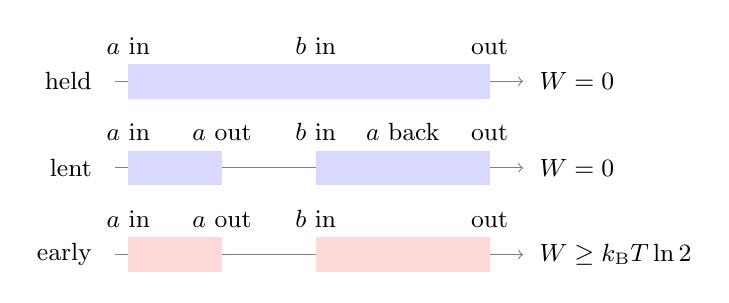
\begin{tikzpicture}[x=0.85cm,y=0.55cm,font=\small]
\node[anchor=east] at (0.6,4.4) {held};
\draw[->,gray] (0.8,4.4) -- (6.9,4.4);
\fill[blue!15] (1.0,4.0) rectangle (6.4,4.8);
\node[above] at (1.0,4.8) {$a$ in}; \node[above] at (3.8,4.8) {$b$ in}; \node[above] at (6.4,4.8) {out};
\node[anchor=west] at (7.0,4.4) {$W=0$};
\node[anchor=east] at (0.6,2.4) {lent};
\draw[->,gray] (0.8,2.4) -- (6.9,2.4);
\fill[blue!15] (1.0,2.0) rectangle (2.4,2.8);
\fill[blue!15] (3.8,2.0) rectangle (6.4,2.8);
\node[above] at (1.0,2.8) {$a$ in}; \node[above] at (2.4,2.8) {$a$ out}; \node[above] at (3.8,2.8) {$b$ in}; \node[above] at (5.1,2.8) {$a$ back}; \node[above] at (6.4,2.8) {out};
\node[anchor=west] at (7.0,2.4) {$W=0$};
\node[anchor=east] at (0.6,0.4) {early};
\draw[->,gray] (0.8,0.4) -- (6.9,0.4);
\fill[red!15] (1.0,0.0) rectangle (2.4,0.8);
\fill[red!15] (3.8,0.0) rectangle (6.4,0.8);
\node[above] at (1.0,0.8) {$a$ in}; \node[above] at (2.4,0.8) {$a$ out}; \node[above] at (3.8,0.8) {$b$ in}; \node[above] at (6.4,0.8) {out};
\node[anchor=west] at (7.0,0.4) {$W\ge\kB T\ln2$};
\end{tikzpicture}
\caption{The same task, the same slowness, three schedules. Return $a$, then return $a\oplus b$; shaded bars show when the device can act on its carriers. Holding $a$ until $b$ arrives allows reversible cleanup, and so does lending it, if the observer returns it unmodified before cleanup. Releasing $a$ for good strands a copy of it in the device.}\label{fig:schedules}
\end{figure}

\paragraph{What this settles.} The law below answers questions left open by several lines of work.
\begin{itemize}
\item Faist, Berta and Brand\~ao asked whether thermal operations can implement every channel that does not commute with time evolution, as a channel on all inputs, at its thermodynamic capacity~\cite{FBB19,FBB21}. For a time reference that must come back with its energy and entropy refunded, the answer is now known: in real time, such a clock reaches the optimal real-time rate for every channel~\cite[Thm.~11]{SaveWork}, and in batch, it cannot always reach the capacity~\cite[Thm.~7]{KeepingTime}. In batch, a reference that comes back only in state, without that refund, as an embezzling state does, can lower the battery's work to the capacity or below it, but only by paying the difference from its own free energy, like a second battery; counting that payment, no time reference does better than a returned clock. To pay a fixed amount of work per use while its state comes back within trace distance $\eta$, such a reference needs an energy range plus $\kB T$ times the logarithm of its dimension of at least order $n/\eta$ over $n$ uses~\cite[Cor.~17]{KeepingTime}.
\item Faist, Oppenheim and Renner asked whether thermal operations with a time reference can do what Gibbs-preserving maps do~\cite{FOR15}. For the channel version of their question, and a reference that must be returned, the answer is a formula: a returned clock supplies phase but no net energy, the batch cost of a channel with such a clock can exceed the capacity when the environment cannot carry the channel's energy change, and for Gibbs-preserving channels this condition decides whether the cost is zero~\cite[Thms.~6--7]{KeepingTime}.
\item Whether a channel is thermodynamically free is decidable when outputs may be held~\cite[Sec.~6]{Order}, and undecidable when they must be released, already for generalized dephasing (Schur-multiplier) channels of a fixed dimension~\cite[Thm.~13]{SaveWork}.
\end{itemize}

\section*{The principle}
The free energy of a device $C$ and an output $O$, measured against their Gibbs states, splits across the release:
\begin{equation}\label{eq:split}
D(\rho_{CO}\|\gamma_C\!\otimes\!\gamma_O)=D(\rho_C\|\gamma_C)+D(\rho_O\|\gamma_O)+I(C{:}O).
\end{equation}
Releasing $O$ strands the mutual information $I(C{:}O)$: no later operation on $C$ alone can recover it as work. At a fixed state, the price of releasing is therefore a mutual information~\cite{Order}. A device chooses its own records~\cite{Bennett73}, and for a channel released one use at a time, the extra price at a fixed input is the least such correlation that an exact implementation must leave~\cite[Thms.~1, 11]{SaveWork}; for general schedules, the law below takes the place of this statement.

A device consists of a controller, a mechanical battery and Gibbs reservoirs. Every operation conserves energy, so that the device acts by thermal operations; the controller must return approximately, in its state, energy and entropy; and the battery starts in an energy eigenstate and ends in a fixed level with probability tending to one, with its entropy and its mean absolute deviation from that level growing sublinearly in the number of uses, so that the work is deterministic~\cite{SaveWork,Order}. A schedule lists, for each carrier, when it arrives and when it leaves. In batch, every input arrives before any output leaves; in real time, each output leaves before the next input arrives. Every visit returns the same carrier with the Hamiltonian it arrived with. A loan is a carrier that leaves the device and later comes back; the observer, who may choose its inputs adaptively from released outputs, may act on a lent carrier before returning it. The device's own clock is part of its controller. The lent arm of Fig.~\ref{fig:schedules} adds one assumption that the law does not make: the observer returns $a$ unmodified.

\section*{The law}
For a schedule $\mathcal S$ and a target strategy $\mathcal T$, the input--output behaviour the device must reproduce against adaptive observers, let
\begin{equation}\label{eq:K}
k_{\mathcal S,\varepsilon}(\mathcal T)=\inf_{\text{extensions}}\ \sup_{\text{observers}}\Bigl[\tfrac{\ln2}\beta S(Z|F)+E\Bigr],
\end{equation}
with entropies in bits. The infimum runs over private extensions: circuits that follow the schedule, reproduce $\mathcal T$ within error $\varepsilon$ against every observer, and need not conserve energy. $Z$ is everything the observer holds at the end, $F$ an inert purification of the extension's initial state, so that $S(Z|F)$ is the entropy the implementation adds to its own record, and $E$ is the energy handed to the observer. For schedules in which every visit closes within the block, and for borrowed resources that start uncorrelated with the controller, the optimal rate of deterministic work is the rate of~\eqref{eq:K}, regularized over many uses as $\varepsilon\to0$~\cite[Thm.~1]{Order}. The rate is attained in batch for time-covariant channels~\cite{FBB21} and for every channel with a returned clock~\cite{KeepingTime}, in real time~\cite{SaveWork}, for interactive processes~\cite{Answering}, and for general schedules by the construction of~\cite{Order}, using the physical modules of~\cite{Answering}. Landauer's bound, the thermodynamic capacity of time-covariant channels, those that commute with the time evolution, with input and output on one system~\cite{FBB19,FBB21}, the real-time cost of channels~\cite{SaveWork}, the cost of interactive processes~\cite{Answering} and the batch cost of a channel whose clock must be returned~\cite{KeepingTime} are the law on special schedules.

\section*{Does answering promptly cost more?}
The task of Fig.~\ref{fig:schedules} pays because it has memory: its late output depends on an early input. A memoryless channel has no such link between uses, so one might expect that releasing its outputs one by one costs nothing extra. For classical channels this is right; for quantum channels it is not. For $n$ uses of a channel $\Phi$ released one by one, the law gives the rate~\cite[Thms.~1, 11]{SaveWork}
\begin{equation}\label{eq:kappa}
\kappa_\beta=\sup_\rho\Bigl[S(\rho)-S(\Phi\rho)+m_\rho+\tfrac{\beta}{\ln2}\Tr H(\Phi\rho-\rho)\Bigr]
\end{equation}
in bits, that is, in units of $\kB T\ln2$, where $m_\rho$ is the infimum, over exact dilations, of the mutual information left between a released output and the device. For a time-covariant channel, waiting for all outputs gives the same expression with $m_\rho=0$, the capacity of Faist, Berta and Brand\~ao~\cite{FBB21}. For a classical channel, one that measures in an energy eigenbasis and prepares diagonal states, the supremum is attained on energy-diagonal inputs, where $m_\rho=0$: the device writes each output as a function of the input and a random seed and hides the seed in a bath, which ends almost independent of the output. A classical channel therefore never saves work by waiting~\cite[Thm.~2]{SaveWork}. A quantum channel can: partial reset of a qubit pays a surcharge at every temperature, and a real-time device implementing the Werner--Holevo channel, a qutrit channel with zero Hamiltonian, pays $\kB T\ln3$ per use, however slowly, against essentially nothing in batch~\cite[Thms.~2--3]{SaveWork}. Processes with memory, like the task of Fig.~\ref{fig:schedules}, pay even when they are classical. These costs are related to the modularity dissipation of information ratchets~\cite{BMC18} and to the online cost of agents executing classical strategies, which quantum memory can lower~\cite{Thompson25}; for devices with unrestricted memory, the law gives the exact real-time price~\cite[Thms.~1, 9]{Answering}.

Order and speed are separate prices that interact only through the thermal interface. In a collision model in which each thermal contact swaps one cell with a fresh Gibbs qubit, a device that resets its cells along strokes of thermodynamic length $\ell_j$, each starting at most half excited, with $K_j$ contacts each, obeys
\begin{equation*}
W\ \ge\ W^{\rm qs}+\tfrac{\kB T}2\textstyle\sum_j\ell_j^2/K_j,
\end{equation*}
where the slow limit $W^{\rm qs}$ contains the order cost~\cite{Order}. For devices that attain their schedules' optima, the order cost is therefore, as the error vanishes, the difference between the slow-limit intercepts of two schedules~\cite[Sec.~8]{Order}.

\section*{Can one decide whether a channel is free?}
In batch, whether a channel is free is a linear condition~\cite[Sec.~6]{Order}. In real time, a channel is free exactly when it is a limit of thermal operations~\cite[Thm.~9]{SaveWork}, and no algorithm decides this, even for generalized dephasing (Schur-multiplier) channels with exact cyclotomic entries in a fixed dimension $d\ge d_0$~\cite[Thm.~13]{SaveWork}. Under local operations and classical communication, and, for delayed-choice tasks, under incoherent operations, the corresponding questions are decidable~\cite[Sec.~6]{Order}. Choosing what to hold is hard in another way: for the linear task that returns $b\oplus Fa$ after the carriers of $a$ in a set $L$ have left, every exact implementation pays $\operatorname{rank}(F_L)\,\kB T\ln2$ per use, and deciding, given $F$ and $m$, whether some choice of $m$ held carriers lowers it at all is NP-complete, because it asks for a short word in the code spanned by the rows of $F$~\cite[Prop.~3]{Order}.

\section*{What does keeping time cost?}
An operation that does not commute with time evolution needs a phase reference. A finite reference that must come back exactly cannot supply it, unless the battery itself holds a phase reference~\cite{MarvianSpekkens19,LostaglioMuller19},~\cite[Thm.~1]{KeepingTime}; one that comes back approximately, with its energy and entropy refunded, runs every channel in real time at the rate~\eqref{eq:kappa}~\cite[Thm.~11]{SaveWork}. In batch, such a returned clock makes the work per use of every channel
\[
B(\Phi)=\max_{\Psi(\rho)=\Psi(\sigma)}\bigl\{\Tr\rho\Delta+\kB T\ln2\,[S(\sigma)-S(\Phi\sigma)]\bigr\},
\]
with $\Delta=\Phi^*(H)-H$ and $\Psi$ the complementary channel: two inputs can be charged separately for energy and entropy exactly when the environment cannot tell them apart~\cite[Thm.~7]{KeepingTime}. $B$ equals $\kB T\ln2$ times the capacity whenever $\Delta$ lies in the span of the products $A_i^*A_j$ of Kraus operators, so that the environment can carry the energy change; otherwise it can exceed it, even for channels of capacity zero. This concerns thermal operations: Faist, Berta and Brand\~ao reach the capacity of every channel with Gibbs-preserving maps, which they take as free~\cite{FBB21}. A returned clock supplies phase but no net energy: for a gate, the energy it exchanges comes back only on average, as a lottery~\cite[Prop.~3]{KeepingTime}.

The same condition decides how large the clock must be. The generator of the channel's time evolution, $i\sum_iA_i^*\dot A_i$, is exactly $\Delta$, and when it lies outside the span of the $A_i^*A_j$ that evolution can be estimated at the Heisenberg limit~\cite{ZhouJiang21}, as in error-corrected metrology~\cite{DemkowiczCzajkowskiSekatski17,ZhouZhangPreskillJiang18}. With a battery that holds no phase reference, a device that implements such a channel reliably therefore reads its own clock to within $1/n$. Its spread, the mean absolute fluctuation of the clock's log-likelihood relative to its Gibbs state, must then grow at least linearly in $n$, at any work, and at least like $n/\sqrt\eta$ if the clock returns within $\eta$, more for vanishing error~\cite[Prop.~8]{KeepingTime}. When $\Delta$ lies in the span, a clock whose spread grows like $\sqrt n$ suffices in batch at fixed error, though not in general at the optimal work, and no channel that is not time-covariant runs with less~\cite[Prop.~9]{KeepingTime}.

The same asymmetry separates a process from its thermodynamic time reverse. In batch, a Gibbs-preserving qutrit channel costs $0.1547\,\kB T$ per use with a returned clock, while its Petz reverse, the reverse process of fluctuation theorems~\cite{Crooks08}, costs nothing~\cite[Prop.~14]{KeepingTime}.

\section*{Order beyond thermodynamics}
Suppose a qubit $B$ must be released, and afterwards the device's memory $M$ must answer one of two questions, chosen after the release, whose answers fix $B$ in non-commuting bases. Every exact realization has $-S(B|M)=1$~\cite[Lemma~5]{Order}: one qubit of quantum memory must outlive the release. Its price depends on the theory: one ebit per use under one-way communication from the answering party (for a single use, Cope's theorem on extremal assemblages gives one ebit of entanglement of formation~\cite{Cope21}), against zero when $B$ is held, and, for the BB84 pair of bases, an order price of $\kB T\ln2$ per use in thermodynamics at zero Hamiltonian. For two tasks in two theories the order prices form a matrix of rank two, so no exchange rate converts order between theories~\cite[Sec.~7]{Order}.

\section*{Measuring the price of order}
\paragraph{A quantum witness.} Take two qubit carriers $A,B$ with zero Hamiltonian and the process that dephases both inputs and maps $|ab\rangle$ to the Bell state obtained by a Hadamard gate on $A$ followed by a CNOT. Held, it is free: two controlled-$Z$ gates from maximally mixed thermal coins, a Hadamard and a CNOT. Released early, every implementation whose controller, Gibbs reservoirs and sharp battery start independent spends, on the probe described below, a nominal work per episode of at least
\begin{equation}\label{eq:witness}
W\ \ge\ \kB T\ln2\,\bigl[1-h_2(e)-e\log_23-P\bigr],
\end{equation}
where $h_2$ is the binary entropy, $P$ bounds the sum of the changes of the controller's energy and entropy and of the battery's entropy and mean deviation, in units of $\kB T\ln2$, and $e$ is the probability that the outputs leave the two-dimensional space of ideal outputs on this probe~\cite[Prop.~6]{Order}. The probe feeds $A=|0\rangle$, then, after $A$ has left, $B$ entangled with a reference $Q$. Because $B$ and $Q$ are prepared after $A$ has left, and the device never acts on $A$ again, $Q$ ends independent of $A$ and of the device's initial purification, and a mathematical decoder on $Q$ and $A$ shows that the device's entropy must rise by at least $1-S(AB)_{\rm decoded}$. Three local Pauli settings, the stabilizers $X_AX_B$ and $Z_QZ_AZ_B$ and their product, measured as $Z_QY_AY_B$, determine the distribution of the stabilizer outcomes and hence $e$; the first two already bound $e$. At $P=0.025$, \eqref{eq:witness} gives $0.878\,\kB T\ln2$ at $e=1\%$ and stays above $0.05\,\kB T\ln2$ up to about $e=17\%$.

\paragraph{Heat form and certification.} In heat form the bound needs no refund of the controller's energy and no sharp battery, and the probe $B$ may be a uniformly random classical bit: the net heat into a monitored thermal bath is at least $\kB T\ln2\,[S(\rho_A)+S(\rho_B)-H_4(p)-s]$, where $p$ is the distribution of the four joint outcomes of the two stabilizers, $H_4(p)$ is its Shannon entropy, $H_4(p)\le h_2(e)+e\log_23$, and $s$ is the entropy allowed to the controller, the battery and the rest of the hardware~\cite[Prop.~6]{Order}. The Pauli data fix the stabilizer distribution, not the budgets: the budgets, or in heat form $s$ and a calibrated readout, must be certified separately, and a fully accounted control interface is the open step toward an experiment.

\paragraph{A classical witness and the lent control.} For the classical task of Fig.~\ref{fig:schedules}, every early-release implementation, even one with quantum memory, raises the device's entropy by at least $1-h_2(e_1+e_2)$ bits per episode on fair inputs when the two outputs err with probabilities $e_1$ and $e_2$, with $e_1+e_2\le1/2$, and a device that randomizes which output carries the error attains it~\cite[App.~F]{Order}. Experiments that already resolve heat at the scale of $\kB T\ln2$~\cite{Berut12,Jun14} could measure it, once the device's memory and controls are fully accounted for. The lent arm of Fig.~\ref{fig:schedules}, with its two-CNOT construction, is the natural control: it costs nothing in the reversible limit, so what is priced is letting go, not delivering early. The same control exposes the main hazard of such an experiment: any record of $a$ kept in the feedback electronics restores access, and entropy moved into the battery or controller must be counted, since heat into the bath alone can fall below $\kB T\ln2$.

\section*{Outlook}
Landauer's principle made information physical. The order in which information may be touched is physical too: patience removes the price of speed, never the price of order. At a fixed state the price of releasing is a mutual information; for memoryless channels the extra price of releasing is purely quantum; for clocks, the span condition that sets the price also decides whether the clock must be read at the Heisenberg limit; and in real time, whether the price vanishes is undecidable. Any machine that must hand over its results while it computes runs to such a schedule, and, within the contract above, the law gives its minimum work rate. A measurement of the gap between held, lent and released outputs, at equal slowness, would make the order of operations a thermodynamic quantity in the laboratory.

\section*{Code availability}
The four companion papers, with their sources and machine checks, are at
\begin{itemize}
\item \url{https://github.com/Apsiape/price-of-time-order},
\item \url{https://github.com/Apsiape/save-work-by-waiting},
\item \url{https://github.com/Apsiape/answering-in-real-time},
\item \url{https://github.com/Apsiape/price-of-keeping-time}.
\end{itemize}

\section*{How this work was done}
This letter summarizes four companion papers~\cite{Order,SaveWork,Answering,KeepingTime}, which give the full proofs. The work is that of its two authors together with AI models from more than one developer. The authors set the direction throughout: they chose the questions, decided which lines to pursue and which to drop, judged and selected the results, and take full responsibility for every claim; the models did most of the exploration, derivation, computation and drafting. Before a result was kept, a model instance that had not seen its proof, usually from a different developer, first tried to refute it and then audited the proof line by line, with exact computation wherever possible. Each paper then went through several rounds of adversarial review, and AI-assisted literature searches were used to check priority and how we report the work of others. Programs and Lean proofs in the papers' public repositories check their numbers, worked examples and finite cores; each paper's verification notes list what is checked by machine and what is proved only in the text. Reports of these blind checks, made by model instances, are available from the authors on request through the letter's repository, \url{https://github.com/Apsiape/order-not-speed}.

\bibliographystyle{unsrturl}
\bibliography{refs}

\end{document}
